\documentclass[a4paper,12pt,article,firamath]{nsi}

\documentclass[a4paper,12pt,exos,firamath]{nsi}
		
\setminted{fontsize=\small}
\begin{document}
{\large\bfseries \scshape Nom Prénom : \makebox[6cm]{\dotfill}\hfill Heure de passage : \makebox[3cm]{\dotfill}\hfill\\
\vspace{2em}
\hrule
\vspace{2mm}
\begin{center}\titlefont\Huge\color{UGLiBlue} BTS SIO\\
	Sous-épreuve E22 \\ 
    Algorithmique appliquée\\
	Contrôle en Cours de Formation\end{center}
\vspace{2mm}
\hrule}
\vspace{2em}

\begin{encadrecolore}{Déroulement de l'épreuve }{UGLiGreen}
	Cette épreuve de Contrôle en cours de Formation (CCF) se déroule en trois étapes :
\begin{itemize}
	\item \textbf{\'Etape 1 : \'Ecrit (30 minutes)}\par
	Vous devez traiter la partie A du sujet. Pour cette partie, l'ordinateur est interdit mais la calculatrice est autorisée.\\
    
    \textbf{Vous inscrirez vos réponses dans le document réponse à la fin du sujet.}\\
    
    Les algorithmes à écrire peuvent être rédigés en \textbf{langage naturel} ou en \textsc{Python}	mais ni en \textsc{C\#} ni en \textsc{VB.Net}.\\
    
    \textbf{À la fin de l'étape 1, votre document réponse doit être remis à la personne surveillant l'épreuve.} Vous garderez le sujet.
    \item \textbf{\'Etape 2 : sur machine (30 minutes)}\par
	Vous devez traiter la partie B du sujet à l'aide d'un ordinateur. Le langage utilisé est celui travaillé dans l'année, à savoir \textsc{Python}.
	Vous sauvegarderez votre travail sur la clé USB fournie.\par 
	La durée totale pour effectuer les deux premières étapes est exactement d'une heure. \par
	\item \textbf{\'Etape 3 : oral (20 minutes au maximum)}\\
	Cette partie se déroule en deux temps. Tout d'abord, vous disposez de 10 minutes pour présenter votre travail de l'étape 2 puis, au cours des 10 minutes suivantes, un entretien permet de préciser votre démarche.
\end{itemize}	

\textbf{À la fin de l'épreuve le sujet devra être rendu à l'examinateur.}
\end{encadrecolore}
\newpage

\titre{Tri par insertion}
\classe{CCF Algo SIO}
\maketitle
On dispose d'une liste d'entiers \mintinline{python}{lst} que l'on aimerait trier dans l'ordre croissant.\\
Nous allons utiliser l'algorithme de tri par insertion qui consiste à partager la liste en deux parties : la partie de gauche, qui devra à tout moment être triée et la partie de droite, qui comporte les autres éléments, non triés.\\

Au début de l'algorithme, la partie triée est composée seulement du premier élément \mintinline{python}{lst[0]} et la partie non triée du reste, puis
\begin{itemize}
    \item	on prend le premier élément de la partie de droite et on le fait « remonter » dans la partie de gauche en l'échangeant au fur et à mesure, jusqu'à ce qu'il soit à sa place ;
    \item	la partie de gauche est triée et comporte un élément de plus, celle de droite comporte un élément de moins ;
    \item   on recommence ceci jusqu'à ce que la partie de droite soit vide.
\end{itemize}
Voici un exemple :
\begin{center}
    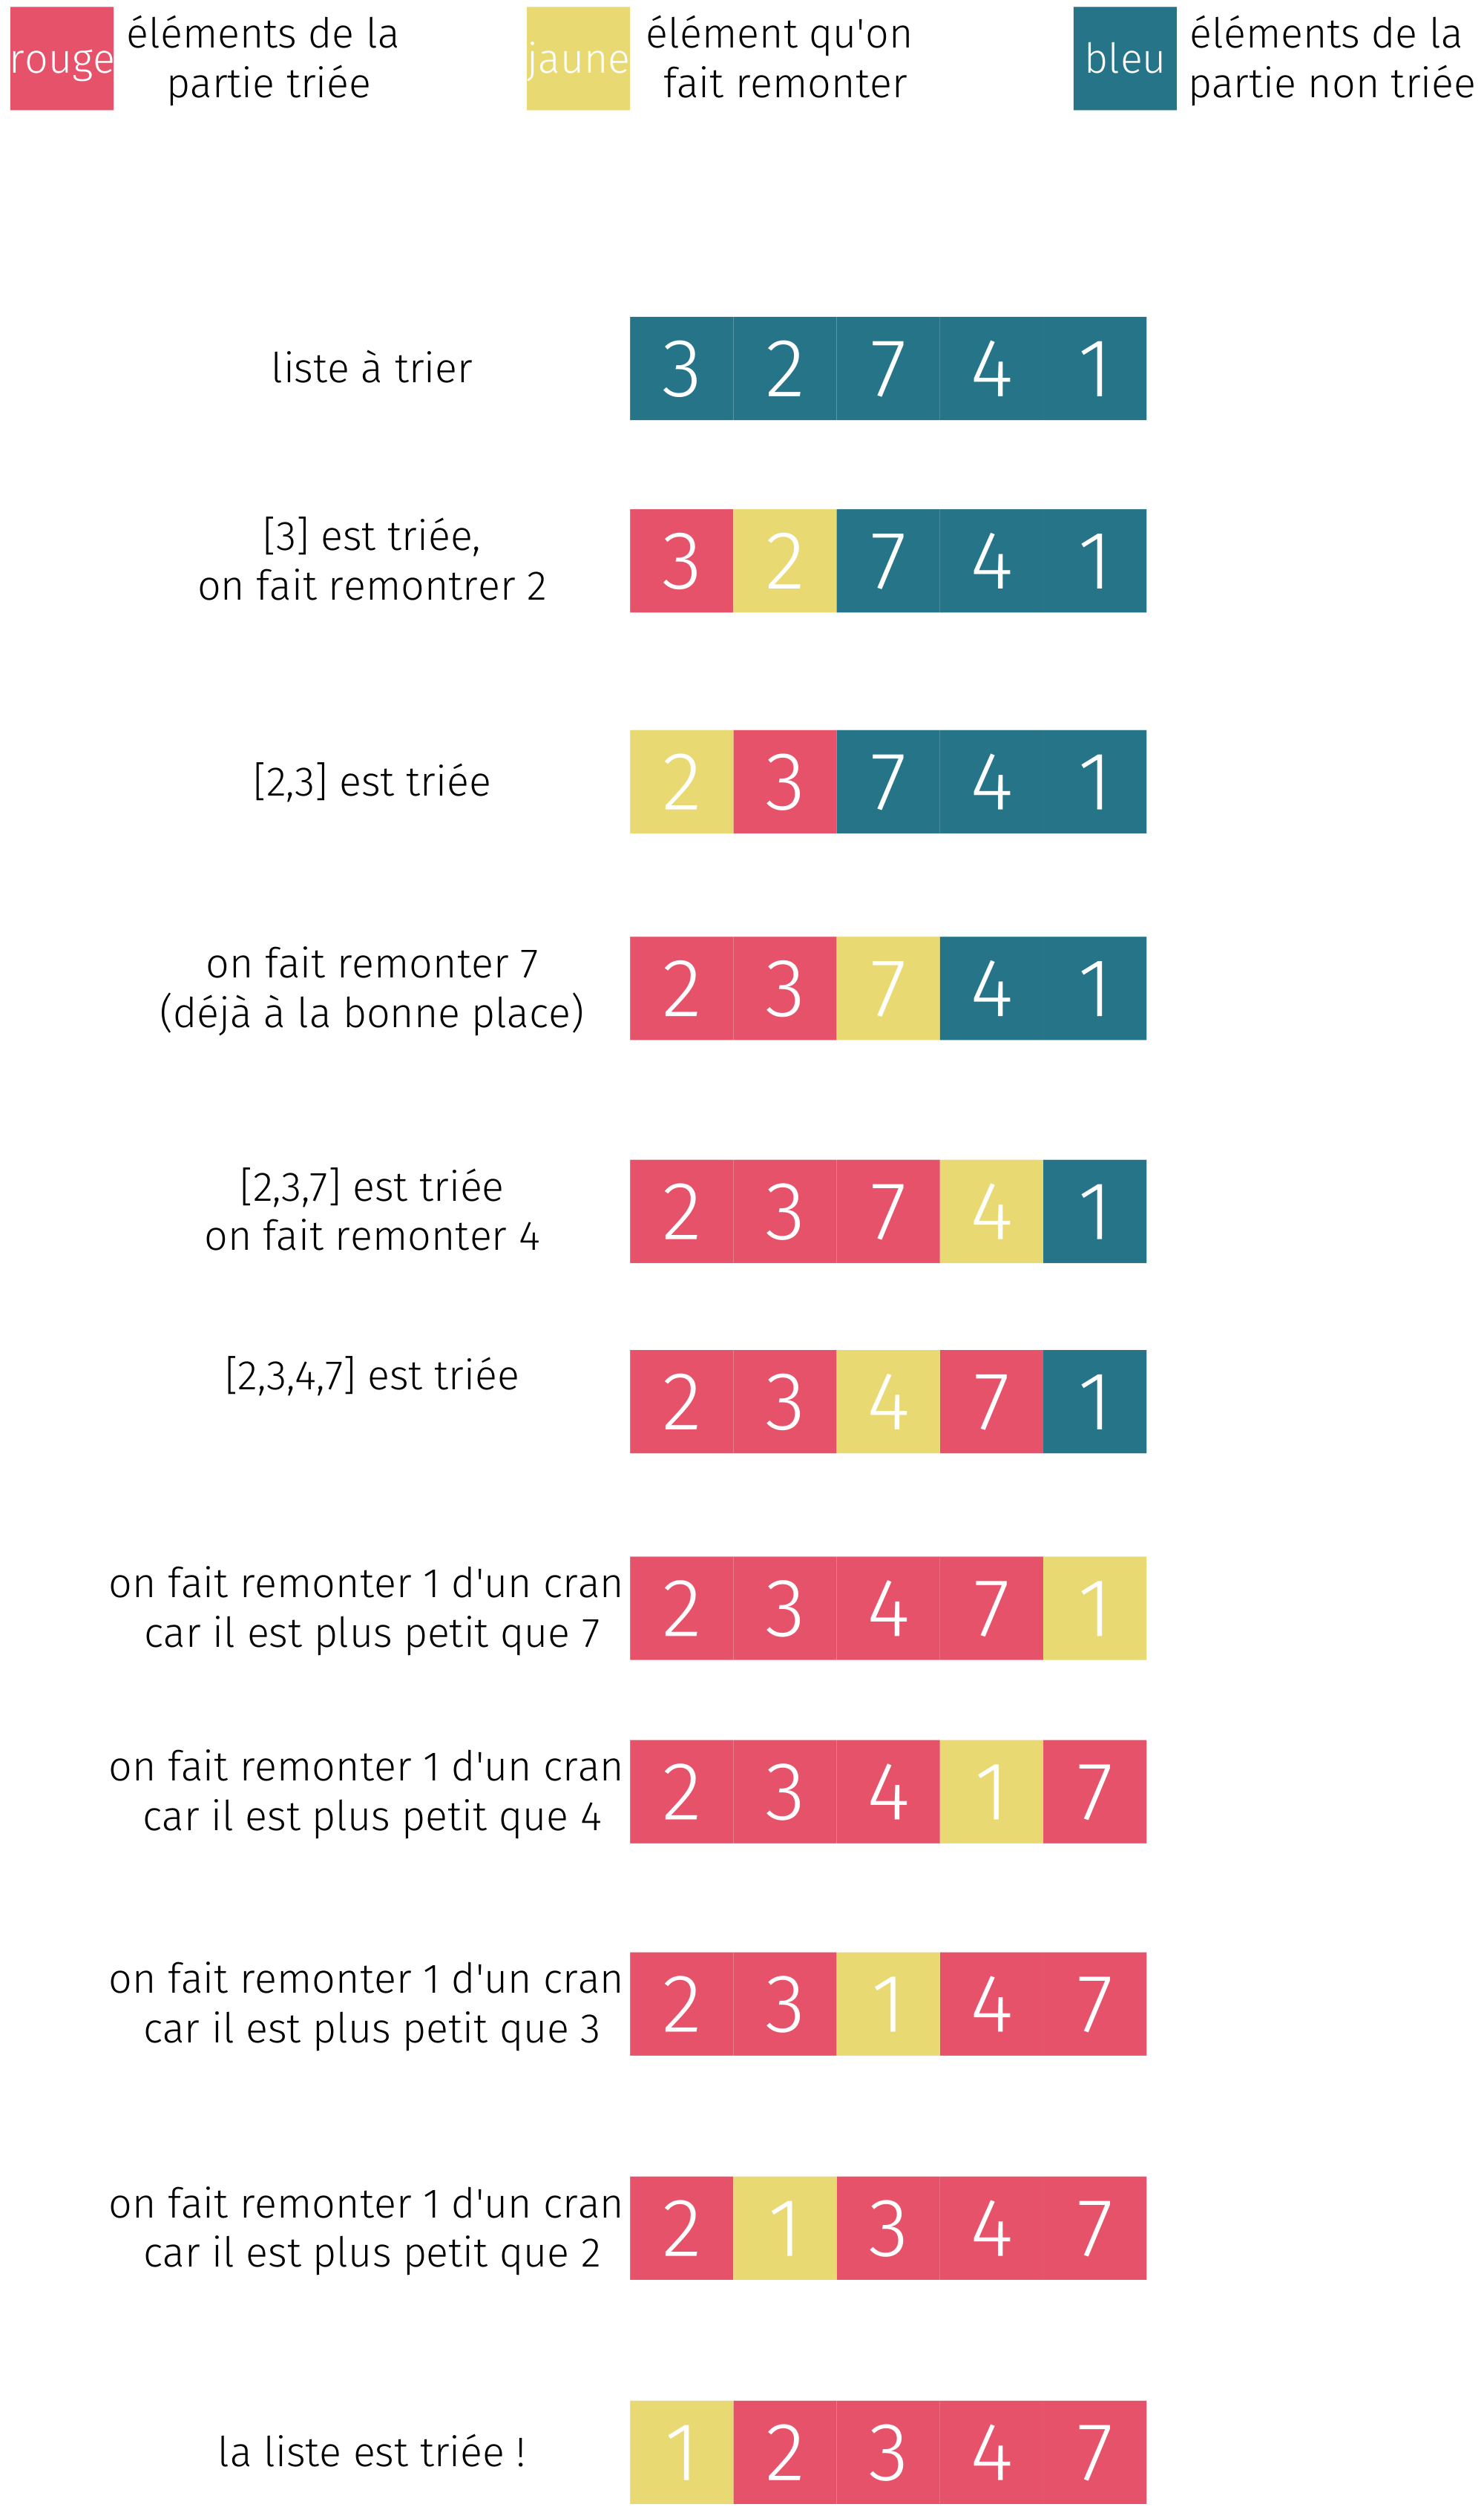
\includegraphics[width=8.7cm]{img/insertion.png}
\end{center}

\begin{questionnum}
    Applique cet algorithme étape par étape en faisant comme à l'exemple précédent avec \mintinline{python}{lst = [4, 2, 8, 0, 3]}
\end{questionnum}

On a commencé à écrire l'algorithme de la fonction \mintinline{python}{insere} qui
\begin{itemize}
    \item	en entrée prend une liste \mintinline{python}{lst} et un entier \mintinline{python}{i} : les éléments de \mintinline{python}{lst[0]} à \mintinline{python}{lst[i - 1]}  sont triés et on veut faire « remonter » \mintinline{python}{lst[i]} parmi eux ;
    \item	ne renvoie rien mais fait remonter \mintinline{python}{lst[i]} au bon endroit (il échange \mintinline{python}{lst[i]} avec \mintinline{python}{lst[i - 1]} tant que celui-ci existe et est plus grand que \mintinline{python}{lst[i]});
\end{itemize}
Par exemple si \mintinline{python}{lst = [4, 6, 7, 5, 1]} \mintinline{python}{insere(lst ,3)} doit donner une valeur de \mintinline{python}{lst} de \mintinline{python}{[4, 5, 6, 7, 1]}.


\begin{questionnum}
    Complète sur ta copie l'algorithme de la fonction \mintinline{python}{insere} .
    \begin{minted}{pseudocode}
        fonction insere(lst, i)
            variables
                temp : entier
            tant que i < 0 et ... repeter
                temp ← lst[i - 1]
                lst[i - 1] ← ...
                lst[i] ← ...
                i ← ...
            fin tant que 
    \end{minted}
\end{questionnum}

On a commencé à écrire la fonction \mintinline{python}{tri_insertion} qui
\begin{itemize}
    \item	en entrée prend la liste \mintinline{python}{lst} à trier ;
    \item	ne renvoie rien mais trie \mintinline{python}{lst} en appliquant le principe de tri par insertion exposé plus haut.
\end{itemize}

\begin{questionnum}
    Complète sur ta copie l'algorithme de la fonction.
    \begin{minted}{pseudocode}
        fonction tri_insertion(lst)
            variables
                i : entiers
            pour i allant de ... à ... repeter
                ...
            fin pour
    \end{minted}
\end{questionnum}

\section*{Étape 2}

\begin{questionnum}
    Ouvrir le fichier \mintinline{python}{tri_insertion.py} et coder les fonctions manquantes.
\end{questionnum}

\begin{questionnum}
    En s'inspirant de ce qui a été fait, créer une fonction \mintinline{python}{tri_insertion_decroissant} qui trie les listes dans l'ordre décroissant.
\end{questionnum}
\end{document}
